% This file was created with tikzplotlib v0.10.1.post13.
\begin{tikzpicture}

  \definecolor{crimson2554141}{RGB}{255,41,41}
  \definecolor{darkgrey176}{RGB}{176,176,176}
  \definecolor{grey}{RGB}{128,128,128}
  \definecolor{lightgrey204}{RGB}{204,204,204}
  \definecolor{mediumslateblue107107255}{RGB}{107,107,255}
  \definecolor{violet25577255}{RGB}{255,77,255}

  \begin{axis}[
      height=0.4\textheight,
      legend cell align=right,
      legend cell align={left},
      legend pos=north west,
      legend style={  at={(1,1.03)},  anchor=south east},
      legend style={fill opacity=0.95, draw opacity=1, text
      opacity=1, draw=lightgrey204},
      tick align=outside,
      tick pos=left,
      title={Classifier probabilities: cl1 strong, cl1 weak, cl2 weak},
      width=0.95\textwidth,
      x grid style={darkgrey176},
      xmin=-0.79, xmax=7.79,
      xtick style={color=black},
      xtick={0,1,2,3.5,4.5,6,7},
      xticklabels={
        {\(\displaystyle R_x^1, R_y^1\)},
        {\(\displaystyle R_x^0, R_y^1\)},
        {\(\displaystyle R_x^1, R_y^0\)},
        \(\displaystyle R_a^0\),
        \(\displaystyle R_a^1\),
        \(\displaystyle R_b^0\),
        \(\displaystyle R_b^1\)
      },
      y grid style={darkgrey176},
      ylabel style={text width=10cm, align=center},
      ylabel={Probability},
      ymajorgrids,
      ymin=0, ymax=0.75,
      ytick style={color=black}
    ]
    \draw[draw=black,fill=violet25577255,line width=0.24pt] (axis
    cs:-0.4,0) rectangle (axis cs:0.4,0.333333333333333);
    \draw[draw=black,fill=violet25577255,line width=0.24pt] (axis
    cs:0.6,0) rectangle (axis cs:1.4,0.333333333333333);
    \draw[draw=black,fill=violet25577255,line width=0.24pt] (axis
    cs:1.6,0) rectangle (axis cs:2.4,0.333333333333333);
    \draw[draw=black,fill=crimson2554141,line width=0.24pt] (axis
    cs:3.1,0) rectangle (axis cs:3.9,0.4);
    \draw[draw=black,fill=crimson2554141,line width=0.24pt] (axis
    cs:4.1,0) rectangle (axis cs:4.9,0.6);
    \draw[draw=black,fill=mediumslateblue107107255,line width=0.24pt]
    (axis cs:5.6,0) rectangle (axis cs:6.4,0.4);
    \draw[draw=black,fill=mediumslateblue107107255,line width=0.24pt]
    (axis cs:6.6,0) rectangle (axis cs:7.4,0.6);
    \addplot [line width=0.32pt, grey, dashed, forget plot]
    table {%
      2.75 -2.77555756156289e-17
      2.75 0.75
    };
    \addplot [line width=0.32pt, grey, dashed, forget plot]
    table {%
      5.25 -2.77555756156289e-17
      5.25 0.75
    };
    \draw (axis cs:0,0.343333333333333) node[
      scale=0.45,
      anchor=south,
      text=black,
      rotate=0.0
    ]{0.33};
    \draw (axis cs:1,0.343333333333333) node[
      scale=0.45,
      anchor=south,
      text=black,
      rotate=0.0
    ]{0.33};
    \draw (axis cs:2,0.343333333333333) node[
      scale=0.45,
      anchor=south,
      text=black,
      rotate=0.0
    ]{0.33};
    \draw (axis cs:3.5,0.41) node[
      scale=0.45,
      anchor=south,
      text=black,
      rotate=0.0
    ]{0.40};
    \draw (axis cs:4.5,0.61) node[
      scale=0.45,
      anchor=south,
      text=black,
      rotate=0.0
    ]{0.60};
    \draw (axis cs:6,0.41) node[
      scale=0.45,
      anchor=south,
      text=black,
      rotate=0.0
    ]{0.40};
    \draw (axis cs:7,0.61) node[
      scale=0.45,
      anchor=south,
      text=black,
      rotate=0.0
    ]{0.60};
    \draw (axis cs:1,-0.09) node[
      scale=0.55,
      anchor=north,
      text=black,
      rotate=0.0
    ]{\bfseries cl1 strong};
    \draw (axis cs:4,-0.09) node[
      scale=0.55,
      anchor=north,
      text=black,
      rotate=0.0
    ]{\bfseries cl1 weak};
    \draw (axis cs:6.5,-0.09) node[
      scale=0.55,
      anchor=north,
      text=black,
      rotate=0.0
    ]{\bfseries cl2 weak};
  \end{axis}

\end{tikzpicture}
